\documentclass[11pt]{article}

\usepackage[margin=1in]{geometry}
\usepackage[T1]{fontenc}
\usepackage{lmodern}
\usepackage{microtype}
\usepackage{booktabs}
\usepackage{array}
\usepackage{multirow}
\usepackage{float}
\usepackage{graphicx}
\usepackage{amsmath,amssymb}
\usepackage{xcolor}
\usepackage[numbers,sort&compress]{natbib}
\usepackage[hidelinks]{hyperref}
\usepackage{url}

\hypersetup{
  pdftitle={NEDOQwen: An Auditable Low-Cost Diagnosis-and-Repair Study for a Turkish-Centric 0.824B Language Model},
  pdfauthor={Ahmet Rıfat Öztürk; Yağız Ekrem Dalar; Ömer Faruk Aksoy; Nedim Mutlu Sezer; Feyzi Arda Salihoğlu},
  colorlinks=true,
  linkcolor=black,
  citecolor=black,
  urlcolor=blue
}

\newcommand{\model}{\textsc{NEDOQwen}}
\newcommand{\tmmlu}{TurkishMMLU-sub}
\newcommand{\tumlu}{TUMLU-mini Turkish}
\newcolumntype{L}[1]{>{\raggedright\arraybackslash}p{#1}}
\setlength{\emergencystretch}{2em}

\title{\model: An Auditable Low-Cost\\
Diagnosis-and-Repair Study for a\\
Turkish-Centric 0.824B Language Model}
\author{Ahmet R{\i}fat \"Ozt\"urk \quad Ya\u{g}{\i}z Ekrem Dalar \quad
\"Omer Faruk Aksoy\\
Nedim Mutlu Sezer \quad Feyzi Arda Saliho\u{g}lu\\
\small Ethosoft Research}
\date{Technical Report --- July 2026}

\begin{document}
\maketitle

\begin{abstract}
Small language models can make non-English model development more accessible,
but internal prompt checks and language-specific design choices may obscure
substantial external failures. We present \model, a Turkish-centric
824M-parameter decoder-only research model, as an auditable case study in
low-cost diagnosis and targeted repair. Clean supervised fine-tuning improves
internal Turkish instruction diagnostics, while public Turkish and Turkic
multiple-choice slices reveal weak academic knowledge, tokenizer coverage
limitations, and severe answer-label bias. A 600-step repair stage increases
\tmmlu{} accuracy from 18.11\% to 21.00\% and \tumlu{} accuracy from 21.33\%
to 32.22\% under a common zero-shot answer-label log-probability protocol. An
answer-label-only ablation reaches 19.56\% and 27.00\%, showing that calibration
explains part, but not all, of the observed gains. Prediction distributions
remain strongly concentrated on C and D, and qualitative failures persist.
The contribution is therefore not a state-of-the-art Turkish model, but a
version-aware, low-cost workflow for exposing internal--external evaluation
mismatch, auditing tokenizer behavior, and reporting partial repair without
mistaking benchmark gains for broad competence.
\end{abstract}

\section{Introduction}

Broad multilingual averages can hide failures that matter for an individual
language. This is particularly consequential for morphologically rich and
underrepresented languages, where tokenization, data coverage, instruction
formatting, and evaluation protocol interact in ways that are difficult to
infer from English-centric aggregate scores. Open multilingual models have
expanded language coverage considerably \citep{conneau2020xlmr,scao2022bloom,
yang2024qwen25}, but local researchers still need affordable methods for
testing whether a language-specific model actually behaves as intended.

Turkish is a useful case study. Its agglutinative morphology and language-
specific characters place pressure on vocabulary construction and fallback
segmentation. A tokenizer that appears linguistically motivated may still have
coverage gaps, while a model that performs acceptably on local instruction
prompts may fail external knowledge and answer-selection tests.

We use \model, a custom 824,256,000-parameter Turkish-centric decoder-only
model, to study a complete diagnose-and-repair loop. The loop combines
tokenizer analysis, internal generation diagnostics, external Turkish/Turkic
benchmark slices, targeted repair, an answer-label-only ablation, prediction-
distribution analysis, regression checks, and explicit limitation reporting.
Our purpose is methodological and artifact-oriented. We do not claim that the
model is state of the art, reliable, production-ready, or generally competent
in Turkish.

This report makes four contributions:
\begin{enumerate}
  \item It presents a version-aware account of a Turkish-centric small-model
  artifact and separates publicly released checkpoints from the later
  experimental checkpoints used in the main results.
  \item It measures tokenizer coverage rather than assuming language-specific
  tokenization is superior, finding nonzero unknown-token behavior and weaker
  compactness than Qwen2.5 on \tmmlu{} text.
  \item It documents a mismatch between improved internal Turkish instruction
  diagnostics and weak external benchmark behavior, including severe answer-
  label skew.
  \item It evaluates a small targeted repair stage, calibration-only ablation,
  contamination controls, uncertainty, qualitative failures, and observed
  compute cost.
\end{enumerate}

\section{Related Work}

\paragraph{Multilingual models and evaluation.}
Multilingual encoders and generators demonstrate cross-lingual transfer, yet
performance remains uneven across languages and tasks
\citep{conneau2020xlmr,scao2022bloom,yang2024qwen25}. TurkishMMLU provides
school-like Turkish multitask questions \citep{yuksel2024turkishmmlu}, while
TUMLU evaluates native Turkic-language understanding \citep{isbarov2025tumlu}.
We use public slices from these resources as diagnostic instruments, not as
official leaderboard submissions. TR-MMLU is relevant but is not reported
because the likely official endpoint tested during the project required
authorization \citep{bayram2025trmmlu}.

\paragraph{Tokenization for morphologically rich languages.}
Subword methods such as BPE and SentencePiece are foundational to modern NLP
\citep{sennrich2016bpe,kudo2018sentencepiece}. Language-aware segmentation may
offer interpretable units, but coverage, normalization, fallback behavior, and
vocabulary construction remain empirical questions. We therefore report both
token compactness and unknown-token rates.

\paragraph{Targeted post-training and benchmark leakage.}
Post-training can repair task-following failures while also teaching benchmark
style. We distinguish exact row-content overlap from style-level transfer.
The repair intentionally teaches generic answer-label and short-format
behavior; therefore, improved multiple-choice performance cannot be treated as
independent evidence of broad knowledge.

\section{Artifact and Version Lineage}
\label{sec:lineage}

Version identity is essential to interpreting this project. Table
\ref{tab:lineage} separates the public releases from the evaluated
experimental line.

\begin{table}[t]
\centering
\small
\begin{tabular}{L{2.3cm}L{4.0cm}L{2.0cm}L{3.4cm}}
\toprule
\textbf{Line} & \textbf{Stage} & \textbf{Public?} & \textbf{Role} \\
\midrule
Public & base pretraining, step 5000 & Yes & released base checkpoint \\
Public & clean-20K SFT from base-5000 & Yes & released instruction checkpoint \\
Experimental & base step 9000 $\rightarrow$ clean-20K SFT & No public release & pre-repair evaluation checkpoint \\
Experimental & answer-label-only repair-600 & No & calibration ablation \\
Experimental & full repair-v2-600 & No & headline post-repair checkpoint \\
\bottomrule
\end{tabular}
\caption{Checkpoint lineage. The benchmark results in this report belong to
the experimental step-9000/repair line and must not be attributed to the
currently public base-5000 or SFT-5000 checkpoints.}
\label{tab:lineage}
\end{table}

The public base model and clean-SFT model are available on Hugging Face
\citep{nedoqwenbase,nedoqwensft}. Their architecture matches the local
experiment registry, but their weights are not the exact weights used for the
headline repair experiments. This distinction is a current reproducibility
limitation, not a cosmetic naming issue.

\section{Model, Tokenizer, and Training Data}

\subsection{Architecture}

\model{} is implemented in custom PyTorch rather than the Transformers
\texttt{AutoModel} interface. It uses rotary positional embeddings
\citep{su2021roformer}, RMSNorm \citep{zhang2019rmsnorm}, SwiGLU feed-forward
blocks, grouped-query attention, and no embedding tying. Table
\ref{tab:architecture} summarizes the configuration verified in both local and
public metadata.

\begin{table}[t]
\centering
\small
\begin{tabular}{ll@{\hspace{1.2cm}}ll}
\toprule
Parameters & 824,256,000 & Layers & 24 \\
Vocabulary & 65,536 & Hidden size & 1,536 \\
Attention heads & 16 & KV heads & 8 \\
MLP dimension & 4,096 & Context & 1,024 \\
Position & RoPE & Normalization & RMSNorm \\
Activation & SwiGLU & Embedding tying & No \\
\bottomrule
\end{tabular}
\caption{NEDOQwen architecture.}
\label{tab:architecture}
\end{table}

\subsection{Pretraining and supervised fine-tuning data}

The released tokenized corpus is a 60.95B-token Turkish web-corpus snapshot
encoded as 32 uint16 shards \citep{nedocorpus}. Its card describes a
FineWeb/FineWeb2/Common-Crawl-style source and cites FineWeb
\citep{penedo2024fineweb}. The released base-5000 model metadata records only
1,310,720,000 tokens seen. We therefore distinguish the size of the available
corpus snapshot from the training exposure of a particular checkpoint.

The public SFT dataset contains a recommended 20,000-example clean subset and a
broader 104,078-example mixture \citep{nedosftdata}. The clean subset derives
from listed Turkish instruction and finance-instruction resources. Upstream
license verification remains necessary before broad redistribution or
commercial use.

\subsection{Tokenizer coverage}

The typed Turkish tokenizer has a 65,536-entry vocabulary. On 5,000 clean SFT
examples it yields 3.0008 tokens per word and a 0.8152\% micro UNK rate. On
\tmmlu{} question-and-choice text, its UNK rate rises to 2.1433\% and its
compactness is weaker than Qwen2.5 and Trendyol-LLM (Table
\ref{tab:tokenizer}). This is an informative negative result: Turkish-aware
design does not guarantee robust coverage.

\begin{table}[t]
\centering
\small
\begin{tabular}{llrrr}
\toprule
\textbf{Text} & \textbf{Tokenizer} & \textbf{Tok/word} & \textbf{UNK \%} & \textbf{UNK n} \\
\midrule
Clean SFT & NEDO 65K & 3.0008 & 0.8152 & 5,909 \\
\tmmlu{} & NEDO 65K & 2.2400 & 2.1433 & 3,106 \\
\tmmlu{} & Qwen2.5 & 1.9436 & 0.0000 & 0 \\
\tmmlu{} & Trendyol-LLM & 2.1137 & 0.0000 & 0 \\
\tmmlu{} & Phi-3.5 & 3.0358 & 0.0000 & 0 \\
\bottomrule
\end{tabular}
\caption{Tokenizer comparison on clean SFT and \tmmlu{} text.}
\label{tab:tokenizer}
\end{table}

\begin{figure}[htbp]
\centering
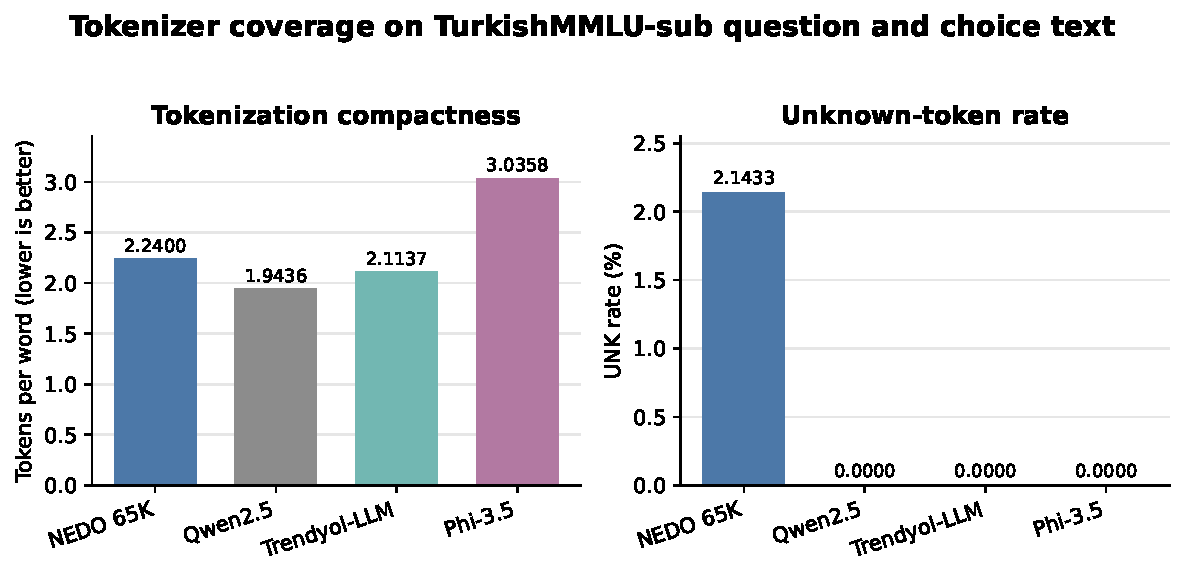
\includegraphics[width=\textwidth]{figures/figure_3_tokenizer_coverage.pdf}
\caption{Tokenizer compactness and unknown-token rate on \tmmlu{} question
and choice text. The Turkish-aware NEDO 65K tokenizer is less compact than
Qwen2.5 and Trendyol-LLM on this slice and is the only compared tokenizer with
a nonzero UNK rate. These measurements are coverage diagnostics and do not
establish a causal relationship with model accuracy.}
\label{fig:tokenizer}
\end{figure}

Accuracy is not monotonic across UNK-count buckets. For pre-repair and
post-repair respectively, accuracy is 15.68\% and 17.80\% for zero UNKs;
17.15\% and 21.68\% for one or two; 17.84\% and 23.24\% for three to five;
and 23.53\% and 21.76\% for six or more. UNK behavior is therefore a coverage
diagnostic, not a demonstrated causal explanation for benchmark errors.

\section{Diagnosis and Repair Protocol}

\subsection{Internal diagnostics}

The project uses 48- and 220-prompt Turkish suites to diagnose expected-answer
matching, repetition, and obviously bad outputs. On the larger suite, moving
from base step 9000 to clean SFT raises the expected score from 0.187 to 0.341
and reduces bad outputs from 137 to 19. However, the same clean-SFT model
remains weak on external benchmarks, demonstrating that internal prompt gains
do not establish general capability.

After full repair, expected match remains essentially stable at 0.339,
repetition changes from 0.088 to 0.090, and bad outputs decrease from 19 to 15.
This is evidence against a large aggregate regression, but not proof of
improved open-ended quality: local summarization, rewriting, translation, and
arithmetic failures remain.

\subsection{External evaluation}

We evaluate 900 examples from \tmmlu{} and 900 Turkish examples from TUMLU-mini
using a common zero-shot plain prompt and answer-label log-probability scoring.
Accuracy is diagnostic and is not necessarily comparable to official
leaderboards or alternative prompting protocols.

\subsection{Repair stage}

The full repair set contains 2,005 targeted examples and 2,000 clean SFT
examples. Major targeted categories are arithmetic (825), answer-letter format
(250), Turkish grammar (240), exact formatting (200), uncertainty calibration
(150), short explanations (150), identity/scope (100), and small stable-fact
categories. Continued SFT runs for 600 steps with learning rate $10^{-5}$,
batch size 2, gradient accumulation 8, and block size 1024.

An answer-label-only repair provides a calibration ablation. The full and
label-only interventions intentionally transfer generic multiple-choice style,
so neither should be interpreted as a task-independent knowledge intervention.

\paragraph{Overlap control.}
The local audit reports zero exact question/choice matches between repair files
and the evaluated benchmark slices. This supports only an exact-string
statement. It does not rule out semantic overlap, upstream contamination, or
format-level transfer. The scan script and output must be released before the
check is independently reproducible.

\section{Results}

\subsection{Benchmark accuracy and ablation}

Table \ref{tab:mainresults} reports the central result. Full repair gives a
small gain on \tmmlu{} and a larger gain on \tumlu{}. The answer-label-only
ablation improves both, demonstrating that calibration is a material part of
the effect. Full repair improves further, especially on TUMLU-mini, but this
does not establish broad reasoning or knowledge.

\begin{table}[t]
\centering
\small
\begin{tabular}{lrrr}
\toprule
\textbf{Model} & \textbf{Params} & \textbf{\tmmlu{}} & \textbf{\tumlu{}} \\
\midrule
Random reference & --- & $\sim$20.00 & $\sim$25.00 \\
Qwen2.5-0.5B-Instruct & 0.5B & 19.33 & 19.89 \\
NEDO pre-repair & 0.824B & 18.11 & 21.33 \\
NEDO label-only repair & 0.824B & 19.56 & 27.00 \\
NEDO full repair-600 & 0.824B & \textbf{21.00} & \textbf{32.22} \\
Qwen2.5-1.5B-Instruct & 1.5B & 28.67 & 42.00 \\
\bottomrule
\end{tabular}
\caption{Accuracy (\%) under the common zero-shot answer-label log-probability
diagnostic protocol.}
\label{tab:mainresults}
\end{table}

\begin{figure}[htbp]
\centering
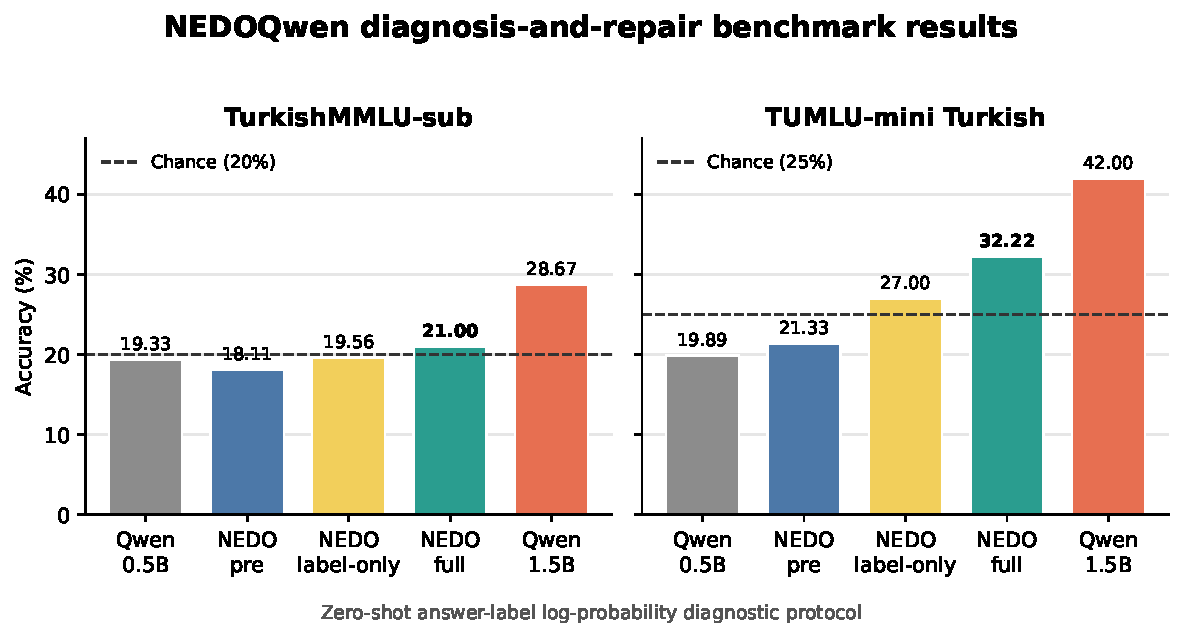
\includegraphics[width=\textwidth]{figures/figure_1_benchmark_accuracy.pdf}
\caption{NEDOQwen diagnosis-and-repair results under the common diagnostic
protocol. Full repair improves \tmmlu{} from 18.11\% to 21.00\% and \tumlu{}
from 21.33\% to 32.22\%. The model remains below Qwen2.5-1.5B-Instruct, and the
\tmmlu{} gain is small. Dashed lines show the chance reference.}
\label{fig:benchmark}
\end{figure}

Paired row-level estimates give a full-minus-pre difference of +2.889
percentage points on \tmmlu{} with a 95\% bootstrap interval of
[0.222, 5.556] and approximate sign-flip $p\approx0.05$. For \tumlu{}, the
difference is +10.889 points with interval [7.778, 14.000] and approximate
$p<0.001$. The former should be described as small and borderline; the latter
is larger under this specific protocol.

\subsection{Prediction-label distributions}

Accuracy alone hides severe answer-label skew. Before repair, C accounts for
85.9\% of predictions on \tmmlu{} and 84.4\% on \tumlu{}. Full repair reduces
C-only collapse but shifts almost all probability mass to C and D (Table
\ref{tab:labels}). Thus, the model remains poorly calibrated even after its
accuracy improves.

\begin{table}[t]
\centering
\small
\begin{tabular}{llrrrrr}
\toprule
\textbf{Benchmark} & \textbf{Stage} & \textbf{A} & \textbf{B} & \textbf{C} & \textbf{D} & \textbf{Acc.} \\
\midrule
\multirow{3}{*}{\tmmlu{}}
 & Pre & 2.3 & 0.1 & 85.9 & 11.7 & 18.11 \\
 & Label-only & 1.9 & 0.1 & 64.6 & 33.3 & 19.56 \\
 & Full & 0.0 & 0.0 & 47.6 & 51.6 & 21.00 \\
\midrule
\multirow{3}{*}{\tumlu{}}
 & Pre & 2.1 & 0.1 & 84.4 & 13.3 & 21.33 \\
 & Label-only & 2.4 & 0.0 & 63.3 & 34.2 & 27.00 \\
 & Full & 0.0 & 0.0 & 45.4 & 54.6 & 32.22 \\
\bottomrule
\end{tabular}
\caption{Predicted answer-label percentages. TUMLU-mini has four choices;
\tmmlu{} also includes E, which remains at or below 0.9\% and is omitted for
compactness.}
\label{tab:labels}
\end{table}

\begin{figure}[htbp]
\centering
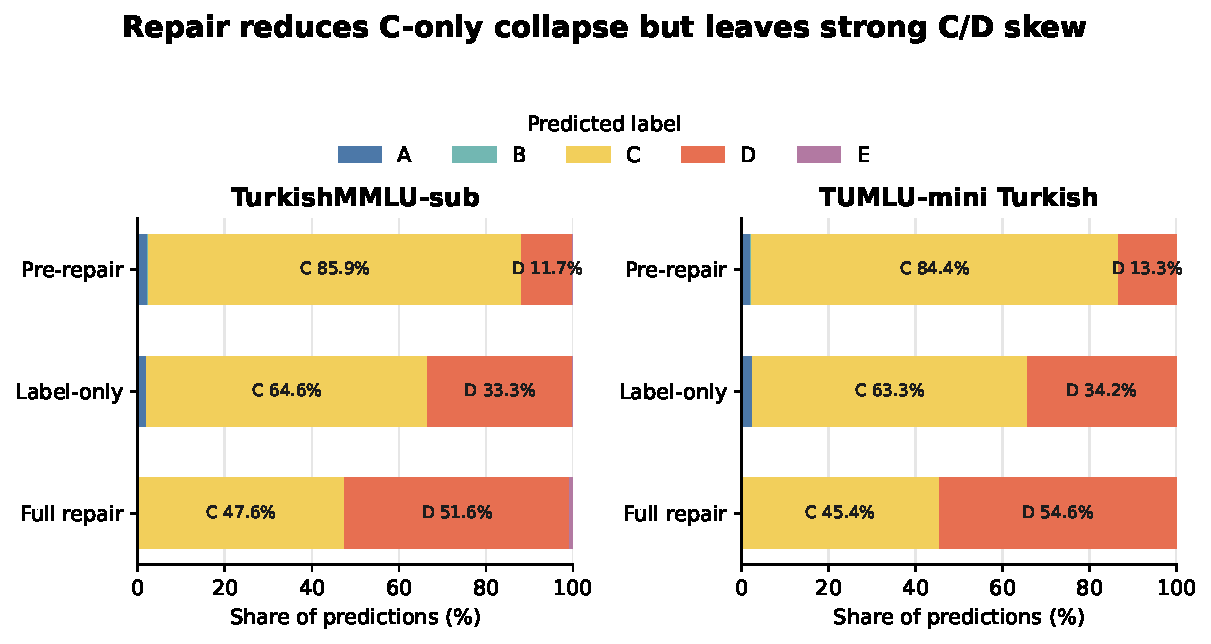
\includegraphics[width=\textwidth]{figures/figure_2_label_distributions.pdf}
\caption{Prediction-label distributions before repair, after answer-label-only
repair, and after full repair. Repair reduces extreme C-only collapse but
leaves strong C/D concentration, showing that increased accuracy does not
eliminate answer-label bias.}
\label{fig:labels}
\end{figure}

\subsection{Protocol sensitivity and qualitative behavior}

A 200-example \tmmlu{} sanity check with repair-600 scores 23.0\% with the
original prompt and choices, 18.0\% with a terse prompt, 23.5\% with original
prompt and shuffled choices, and 21.5\% with terse prompt and shuffled choices.
The prediction distribution changes strongly with wording. We therefore treat
all benchmark values as protocol-sensitive diagnostics.

Sixteen before/after examples show that repair often reduces pathological
repetition and sometimes improves format control. They also show unchanged
errors and local regressions: arithmetic remains unreliable, translation is
weak, and some summarization or rewriting prompts degrade. Reduced repetition
must not be confused with factual correctness.

\section{Compute and Reproducibility}

Recorded automated benchmark, analysis, and repair jobs total approximately
1,674 seconds, or 0.465 observed GPU-hours. At the project's illustrative rate
of 50 TRY per GPU-hour, this corresponds to about 23.25 TRY; the repair round
itself accounts for about 0.12 GPU-hours and 5.99 TRY. These are project-
specific elapsed-time estimates, not universal infrastructure prices.

The public base checkpoint, public SFT checkpoint, tokenized corpus, and SFT
mixture provide useful partial provenance. The exact evaluated step-9000
clean-SFT, label-only, and repair-v2-600 checkpoints are now identified by
SHA-256, and a privacy-clean package contains evaluation scripts, sanitized
row-level predictions, deterministic uncertainty code, and overlap-scan
results. These materials are not yet public, so full public reproduction
remains pending. We report this limitation directly rather than treating
similarly named releases as substitutes.

\section{Discussion}

\paragraph{Internal diagnostics are necessary but insufficient.}
The large improvement from base to clean SFT on internal prompts does not
predict external academic multiple-choice behavior. Local prompt suites and
external benchmark slices reveal different failure classes and should be used
together.

\paragraph{Language-aware tokenization must be tested empirically.}
The NEDO tokenizer provides typed Turkish segmentation, but it is not more
compact than mature multilingual tokenizers on the evaluated text and has
nonzero unknown-token behavior. Better fallback coverage and vocabulary
construction are more defensible future goals than assuming linguistic design
alone guarantees an advantage.

\paragraph{Repair is partial and format-sensitive.}
The label-only ablation and post-repair prediction distributions show that
answer formatting and calibration account for substantial behavior. Full
repair contributes additional gains, but strong C/D skew and qualitative
failures remain. The workflow is valuable precisely because it prevents a
score increase from being marketed as broad capability.

\paragraph{Version-aware release is part of scientific reporting.}
A public checkpoint with the same architecture or family name is not evidence
that the published experiment is reproducible. Each reported table should map
to exact checkpoint, tokenizer, dataset, config, code, and result revisions.
The present audit makes that gap explicit and defines the artifacts needed to
close it.

\section{Limitations}

The study evaluates one custom Turkish-centric model family and cannot support
general claims about all small or underrepresented-language models. The
external protocol is diagnostic rather than official leaderboard reporting.
Full TurkishMMLU and TR-MMLU are not reported. No formal human evaluation or
deployment study is included. The repair mixtures are synthetic and may teach
benchmark style despite zero detected exact row overlap. Tokenizer correlations
are not causal. Public artifacts do not yet reproduce the exact headline
checkpoint line. The model remains weak, label-biased, sensitive to prompt
wording, non-Transformers-native, and unsuitable for end-user deployment.

\section{Ethics and Responsible Release}

The model and data derive from web and instruction corpora that may contain
noise, bias, outdated information, copyrighted material, or sensitive content.
The tokenized corpus does not retain document-level URLs, limiting provenance
auditing and removal workflows. Upstream licenses and terms for SFT mixtures
require further review. We advise against legal, medical, educational grading,
public-service, safety-critical, or other high-stakes use. A responsible release
must include model and data cards, exact version lineage, benchmark limitations,
label-distribution diagnostics, contamination caveats, and a clear statement
that the artifact is not a reliable Turkish assistant.

\section{Conclusion}

\model{} demonstrates why small non-English models should be evaluated as
auditable systems rather than promoted from a single score. The project finds
that internal instruction gains coexist with weak external behavior; a
Turkish-aware tokenizer still has coverage limitations; targeted repair raises
two diagnostic benchmark scores; calibration explains a material fraction of
the improvement; and severe label skew persists. The resulting contribution
is a low-cost, version-aware diagnosis-and-repair workflow and an honest record
of what remains unsolved.

\bibliographystyle{plainnat}
\bibliography{references}

\appendix

\section{Additional Result Tables}

\begin{table}[H]
\centering
\small
\begin{tabular}{lrrr}
\toprule
\textbf{Comparison} & \textbf{$\Delta$ pp} & \textbf{95\% CI} & \textbf{Approx. $p$} \\
\midrule
TMMLU full $-$ pre & +2.889 & [0.222, 5.556] & 0.050 \\
TUMLU full $-$ pre & +10.889 & [7.778, 14.000] & $<0.001$ \\
TMMLU label $-$ pre & +1.444 & [-0.333, 3.333] & 0.173 \\
TUMLU label $-$ pre & +5.667 & [3.444, 8.111] & $<0.001$ \\
TMMLU full $-$ label & +1.444 & [-0.444, 3.333] & 0.160 \\
TUMLU full $-$ label & +5.222 & [2.889, 7.556] & $<0.001$ \\
\bottomrule
\end{tabular}
\caption{Paired uncertainty estimates from existing row-level outputs.}
\end{table}

\begin{table}[H]
\centering
\small
\begin{tabular}{lrr}
\toprule
\textbf{Subject} & \textbf{\tmmlu{}} & \textbf{\tumlu{}} \\
\midrule
Biology & 25 & 33 \\
Chemistry & 24 & 29 \\
Geography & 18 & 31 \\
History & 22 & 41 \\
Mathematics & 23 & 30 \\
Philosophy & 18 & 33 \\
Physics & 19 & 25 \\
Religion and Ethics & 19 & 36 \\
Turkish / Native Language and Literature & 21 & 32 \\
\bottomrule
\end{tabular}
\caption{Repair-600 subject accuracy (\%). Category names are harmonized for
display; the underlying benchmark taxonomies are not identical.}
\end{table}

\section{Public Artifact URLs}

\begin{itemize}
  \item \href{https://huggingface.co/Ethosoft/nedoqwen_0.8b_base_pretrained}{Base-5000 model repository}
  \item \href{https://huggingface.co/Ethosoft/nedoqwen_0.8b_pretrained_sft}{Public SFT-5000 model repository}
  \item \href{https://huggingface.co/datasets/Ethosoft/nedo-turkish-65k-tokenized-60b}{Tokenized pretraining corpus repository}
  \item \href{https://huggingface.co/datasets/Ethosoft/nedo-turkish-sft-mixtures}{SFT mixtures repository}
\end{itemize}

The exact evaluated step-9000 and repair-v2-600 checkpoint URLs are pending.

\end{document}
